\documentclass[colophon, english]{phduio}

\usepackage{phdstyle}   % Custom style
\usepackage{kantlipsum} % Dummy text

\author{Author}
\title{Working Title}
\subtitle{Optional subtitle}
\department{Department}
\faculty{Faculty}
\affiliation
{
    Optional Second Affiliation
    \and
    Optional Further Specification
}
\ISSN{1234-5678}           % Request correct number from repro@uio.no
\dissertationseries{1234}  % Request correct number from repro@uio.no


\includeonly
{
    sections/dedication,
    sections/preface,
    sections/papers,
    sections/introduction,
    sections/paperI,
    sections/paperII,
    sections/paperIII,
    sections/appendixA,
    sections/appendixB,
}


\begin{document}

    \frontmatter        % Folios in Roman numerals, unnumbered chapters.

    \uiotitle

    \thispagestyle{empty}
\vspace*{\stretch{1}}
\begin{flushright}
    \emph{To my ghostwriter}
\end{flushright}
\vspace*{\stretch{3}}
    \chapter{Preface}


This thesis is submitted in partial fulfillment of the requirements
for the degree of \emph{Philosophiae Doctor} at the University of Oslo.
The research presented here was conducted at the University of Oslo and at CERN,
under the supervision of professor Main Supervisor and associate professor Co Supervisor.
This work was supported by the Norwegian Research Council through grant 123456.

The thesis is a collection of three papers,
presented in chronological order of writing.
The common theme to them is a \LaTeX\ thesis template.
The papers are preceded by an introductory chapter that relates them to each other
and provides background information and motivation for the work.
Two of the papers are joint work with Second Author.
I am the sole author of the remaining paper.


\section*{Acknowledgements}

Thanks for all the fish!


\vskip\onelineskip
\begin{flushleft}
    \sffamily
    % \uiocolon\textbf{\theauthor}
    \textbf{\theauthor}
    \\
    Risø,\MONTH\the\year
\end{flushleft}
    \chapter{List of Papers}


\section*{\cref{pap:first}}
Author, F.\ and Author, S.
\enquote{The First Paper}.
In: \emph{Journal of Universal Rejection}.
Vol.\ 3,
no.\ 2
(2011),
pp.~123--456.
\doi{10.1000/182}.

\section*{\cref{pap:A4}}
Author, F.\ and Author, S.
\enquote{A4 Paper}.
\emph{Submitted for publication.}

\section*{\cref{pap:third}}
Author, F.
\enquote{The Third Paper}.
To appear in \emph{Journal of Universal Rejection}.

    \cleartorecto
    \tableofcontents    % Or \tableofcontents*
    \cleartorecto
    \listoffigures      % Or \listoffigures*
    \cleartorecto
    \listoftables       % Or \listoftables*

    \mainmatter         % Folios in Arabic numerals, numbered chapters.

    \chapter{Introduction}
\label{sec:intro}

\kant[4] % Dummy text
\todo[inline]{Rewrite this!}

\section{Figures and Tables}

% Standalone with \input:
\begin{figure}[htbp]
    \centering
    \documentclass[tikz]{standalone}
\begin{document}
    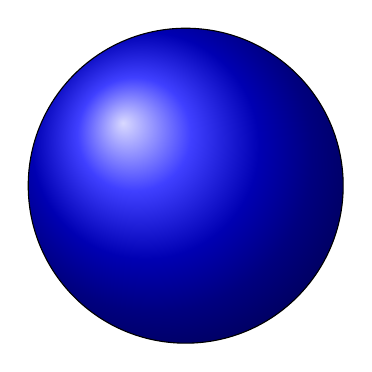
\begin{tikzpicture}
          \draw[shading = ball] (0, 0) circle (2);
    \end{tikzpicture}
\end{document}
    \caption[One ball]{One ball.}
\end{figure}

% Standalone with \includegraphics:
\begin{figure}[thbp]
    \centering
    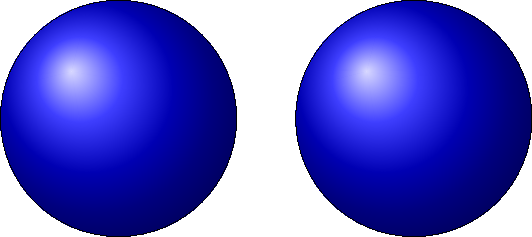
\includegraphics{balls}
    \caption[Two balls]{Two balls.}
\end{figure}

% Todonotes:
\begin{figure}[hbp]
    \centering
    \missingfigure{Three balls.}
    \caption[Three balls]{Three balls.}
\end{figure}

\kant[5-6] % Dummy text

% Booktabs:
\begin{table}[htbp]
    \centering
    \begin{tabular}{@{}ll@{}}
        \toprule
        \textbf{Correct}               & \textbf{Incorrect}      \\
        \midrule
        \( \varphi \colon X \to Y \)   & \( \varphi : X \to Y \) \\[0.5ex]
        \( \varphi(x) \coloneqq x^2 \) & \( \varphi(x) := x^2 \) \\
        \bottomrule
    \end{tabular}
    \caption[Colons]{Proper colon usage.}
\end{table}

\begin{table}[htbp]
    \centering
    \begin{tabular}{@{}ll@{}}
        \toprule
        \textbf{Correct}     & \textbf{Incorrect}         \\
        \midrule
        \( A \implies B \)   & \( A \Rightarrow B \)      \\
        \( A \impliedby B \) & \( A \Leftarrow B \)       \\
        \( A \iff B \)       & \( A \Leftrightarrow B \)  \\
        \bottomrule
    \end{tabular}
    \caption[Arrows]{Proper arrow usage.}
\end{table}

% Tablefootnote and multirow:
\begin{table}[htbp]
    \centering
    \begin{tabular}{@{}ll@{}}
        \toprule
        \textbf{Correct}
        & 
        \textbf{Incorrect}
        \\
        \midrule
        \( -1 \) 
        & 
        -1
        \\[0.3ex]
        1--10
        &
        1-10
        \\[0.3ex]
        Birch--Swinnerton-Dyer\tablefootnote{It is now easy to tell that Birch and Swinnerton-Dyer are two people.} conjecture
        &
        Birch-Swinnerton-Dyer conjecture
        \\[0.3ex]
        The ball \dash which is blue \dash is round.
        &
        \multirow{ 2}{*}{The ball - which is blue - is round.}
        \\[0.3ex]
        The ball---which is blue---is round. 
        &
        \\
        \bottomrule
    \end{tabular}
    \caption[Dashes]{Proper dash usage.}
\end{table}

\begin{table}[hbtp]
    \centering
    \begin{tabular}{@{}*{2}{p{0.5\textwidth}}@{}}
        \toprule
        \textbf{Correct} &  \textbf{Incorrect}
        \\
        \midrule
        \enquote{This is an \enquote{inner quote} inside an outer quote}
        &
        "This is an 'inner quote' inside an outer quote"
        \\
        \bottomrule
    \end{tabular}
    \caption[Quotation marks]
    {Proper quotation mark usage.
    The \texttt{\textbackslash enquote} command chooses the correct
    quotation marks for the specified language.}
\end{table}

\section{Summary of Papers}

\begin{description}
    \item[\cref{pap:first}]
    focuses on the aspects of being the first paper of a thesis,
    following \cref{sec:intro}.

    \item[\cref{pap:A4}]
    demonstrates how illegible the font size becomes when an A4 paper article is shrunk in order to fit into the thesis.

    \item[\cref{pap:third}]
    shows a new and exciting result about the final paper in an article based doctoral thesis.
\end{description}

    \paper              % "Chapter" is renamed "Paper"
    \paperpage          % Similar to \part*{Papers}, but appears in TOC
    \numberofpapers{3}  % Specify size of thumb indices

    \author
{
    First Author\orcid{0000-0000-0000-0000}
    \and
    Second Author
}
\title{The First Paper}
\thanks{The authors were partially supported by CERN.}
\metadata
{
    Published in \emph{Journal of Universal Rejection},
    June~2011,
    volume~3,
    issue~2,
    pp.~123--456.
    \doi{10.1000/182}.
}
\maketitle
\label{pap:first}

\begin{abstract}
    \kant[7]     % Dummy text
\end{abstract}

\startcontents[chapters]
\printcontents[chapters]{}{1}{\section*{\contentsname}}

\section{Introduction}

\gls{GrIS} is the largest ice mass in the Northern Hemisphere.

\kant[8-11]      % Dummy text

\begin{theorem}[{\citep{AM69}}]
    \label{thm:dedekind}
    Let \( A \) be a Noetherian domain of dimension one. Then the following are equivalent:
    \begin{enumerate}
        \item
        \( A \) is integrally closed;

        \item
        Every primary ideal in \( A \) is a prime power;

        \item
        Every local ring \( A_\mathfrak{p} \) \( (\mathfrak{p} \neq 0) \) is a discrete valuation ring.
    \end{enumerate}
\end{theorem}

\begin{acknowledgements}
    The first author was partially supported by The Research Council of Norway.
\end{acknowledgements}

%% Format bibliography like a section, not a chapter:
\printbibliography[heading = subbibliography]
\stopcontents[chapters]

\paragraph{Authors' addresses}
\begin{description}
    \item[First Author]
    University of Oslo,
    Postboks 1337 Blindern, 0316 Oslo, Norway,
    \href{mailto:fauthor@uio.no}{fauthor@uio.no}

    \item[Second Author]
    Oxbridge University,
    221B Baker Street, London NW1 6XE, United Kingdom,
    \href{mailto:second.author@oxbridge.co.uk}{second.author@oxbridge.co.uk}
\end{description}
    \author
{
    First Author
    \and
    Second Author
}
\title{A4 paper}
\metadata{Submitted for publication. \arxiv{1708.04101}.}
\maketitle
\label{pap:A4}


\includearticle{sections/a4paper}
    \author{First Author\protect\footnotemark}
\title{The Third Paper}
\metadata{To appear in \emph{Journal of Universal Rejection}.}
\maketitle
\label{pap:third}

\footnotetext
{%
    University of Oslo,
    Postboks 1337 Blindern, 0316 Oslo, Norway,
    \href{mailto:fauthor@uio.no}{fauthor@uio.no}
}

\begin{abstract}
    \kant[12] % Dummy text
\end{abstract}

\section{First Section}
\kant[13-14]  % Dummy text

\begin{subappendices}             % Appendix for this chapter/paper only
    \section{First Subappendix}
    \label[appendix]{sec:sub-app} % Optional argument: Correct cross reference
    \kant[15]                     % Dummy text
\end{subappendices}

\begin{acknowledgements}
    Thanks to the anonymous referee for pointing out that \cref{sec:sub-app} can be found in \citet{Har77}.
\end{acknowledgements}

%% Format bibliography like a section, not a chapter:
\printbibliography[heading = subbibliography]

    \appendix           % "Chapter" is renamed "Appendix"
    \appendixpage       % Similar to \part*{Appendices}, but appears in TOC

    \chapter{The First Appendix}
\label{app:first-app}
\kant[20-21] % Dummy text
\section{First Section}
\kant[22]    % Dummy text
\section{Second Section}
\kant[23-24] % Dummy text
    \chapter{Source Code}
\label{app:source}
\section{Implementation}
The \texttt{phduio} class is implemented in the following way:
\lstinputlisting[language = {[LaTeX]{TeX}}]{phduio.cls}

\end{document}